\chapter{NEPTUNE\_CFD Simulations of DEBORA Cases}
\label{chap:debora_ncfd}

Due to the large amount of measurements along with its scaling conditions with PWR flows, the DEBORA cases have been often used for validation of multiphase simulation tools, from simple 1D / 2D codes \cite{kledy_DEBORA, gueguen_contribution_2013, manon_contribution_2000} to CFD softwares \cite{mimouni_debora, guelfi_neptune, bestion_debora, baglietto_debora}, helping to conduct separate validation and comparison of several modeling aspects involved in such codes (interfacial heat and momentum transfer, turbulence, interfacial area transport, etc.). 

\npar

In this Chapter, we present neptune\_cfd simulations of the DEBORA experiment. The objective is to assess the current modeling of the code for dispersed two-phase boiling flows. To do so, we will simulate cases from the different campaigns of the DEBORA database (C800 and C3000) to conduct comparisons of void faction, bubble diameter, vapor velocity, liquid temperature and wall temperature profiles.

\npar

As identified in Chapter \ref{chap:debora}, our focus will be on cases from the G2P26W16 series, since they provide the most extensive set of measurements in very close operating conditions.


\section{Simulation Setup}

Since the geometry of the DEBORA experiment presents an axisymmetry, we simplify the simulation setup in order to realize a 2D axisymmetric computation. The computational domain consists of a 1$\degree$ angular section of radius $R=9.6$\ mm and 3.85\ m length (Figure \ref{fig:deb_cfd_domain}).


\begin{figure}[!h]
\centering
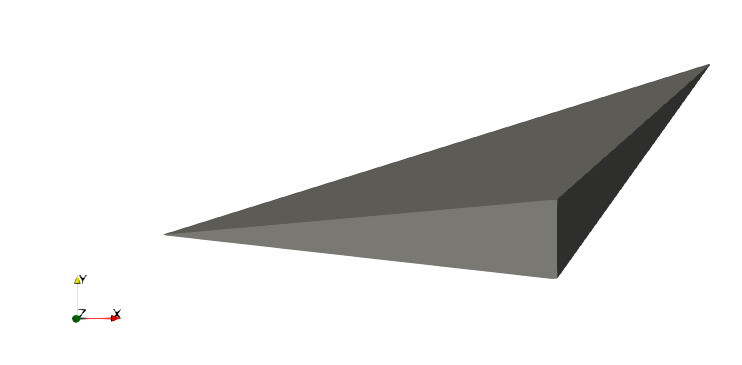
\includegraphics[width=0.6\linewidth]{img/DEBORA/cfd/msh/domain.png}
\caption{View of the computational domain.}
\label{fig:deb_cfd_domain}
\end{figure}


The boundary conditions are:

\begin{itemize}
\item Uniform heat flux for $0.2$\ m $\leq z \leq$ 3.5\ m ;
\item Adiabatic wall for $z<0.2$\ m and $z>3.7$\ m ;
\item Uniform outlet pressure ;
\item Uniform inlet velocity ;
\item Symmetry condition on remaining faces.
\end{itemize}

The inlet section before heating is approximately $10D_{h}$ long and the extracted radial profile for comparisons is located at the end of the heating length. The angular section consists of 1 mesh while radial and axial direction are uniformly discretized. Four meshes are considered, presented on Table \ref{tab:deb_cfd_msh} and Figure \ref{fig:deb_cfd_msh_rad}.



\begin{table}[!h]
\centering

\begin{tabular}{c||c|c|c|c}
Mesh name & M1 & M2 & M4 & M8  \\
\hline
Number of cells (radial $\times$ axial) & 10  $\times$ 100 & 20 $\times$ 200 & 40 $\times$ 400 & 80 $\times$ 800
\end{tabular}

\caption{Mesh parameters}
\label{tab:deb_cfd_msh}

\end{table}

\npar

\begin{figure}[!h]
\centering
\subfloat[Mesh M1]{
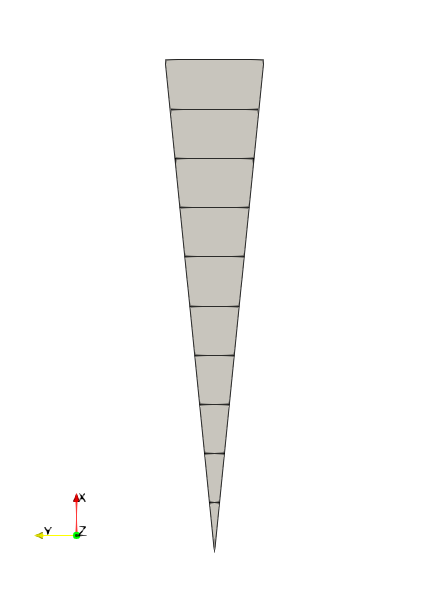
\includegraphics[width=0.25\linewidth]{img/DEBORA/cfd/msh/deb_m1.png}
}
\subfloat[Mesh M2]{
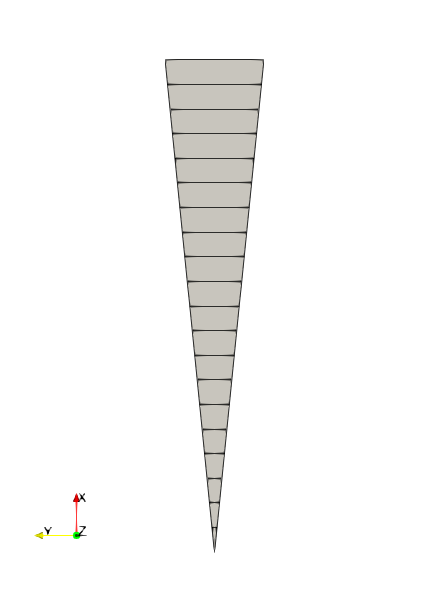
\includegraphics[width=0.25\linewidth]{img/DEBORA/cfd/msh/deb_m2.png}
}
\subfloat[Mesh M4]{
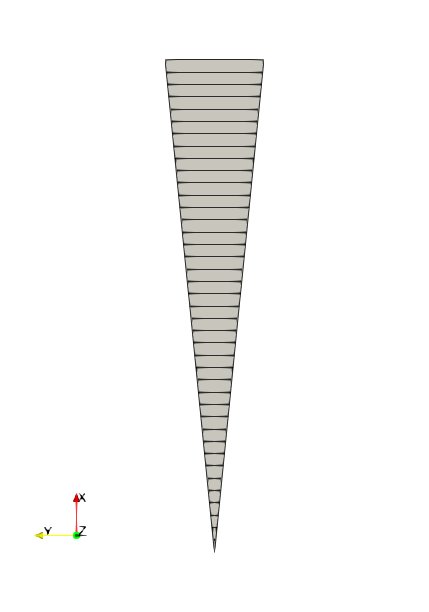
\includegraphics[width=0.25\linewidth]{img/DEBORA/cfd/msh/deb_m4.png}
}
\subfloat[Mesh M8]{
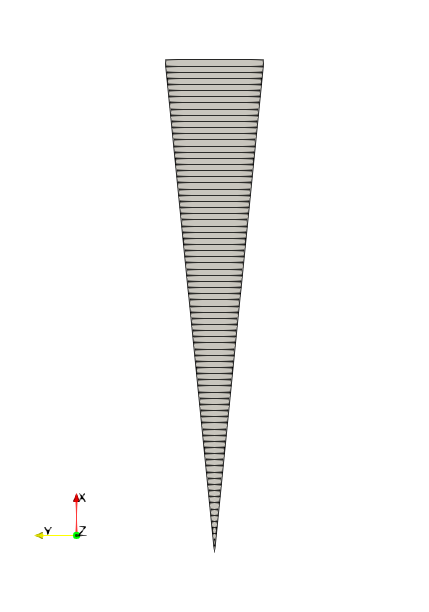
\includegraphics[width=0.25\linewidth]{img/DEBORA/cfd/msh/deb_m8.png}
}
\caption{View of the radial meshes.}
\label{fig:deb_cfd_msh_rad}
\end{figure}


\npar

The computation runs using the transient solver of NCFD for a long enough physical time ensuring temporal stabilization and convergence of the results. 

\begin{note*}{}
First simulated case was simulated up to a physical time of 40\ s, ensuring the time-convergence. Further simulations used this first case as a restart point, allowing to reach time-convergence in less than 10\ s when changing boundary conditions.  
\end{note*}



\section{Mesh Sensitivity Study}

On Figure \ref{fig:deb_cfd_msh_sensi}, we present simulation results for the 4 meshes (Table \ref{tab:deb_cfd_msh}) of the case 30G2P26W16Te66.6. 

\begin{figure}[!h]
\centering
\subfloat[Void fraction]{
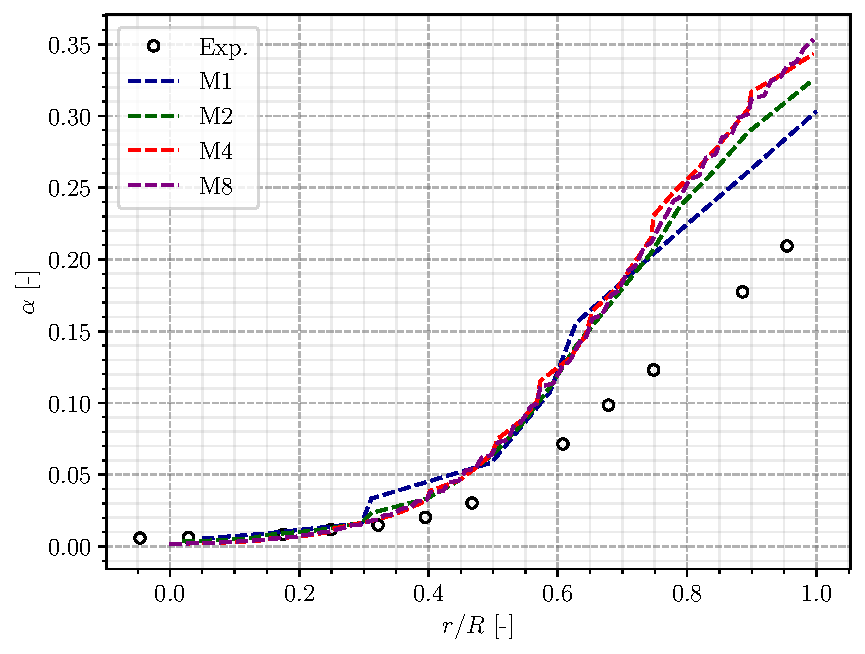
\includegraphics[width=0.5\linewidth]{img/DEBORA/cfd/30G2P26W16/30T66_alpha_msh.pdf}
}
\subfloat[Bubble diameter]{
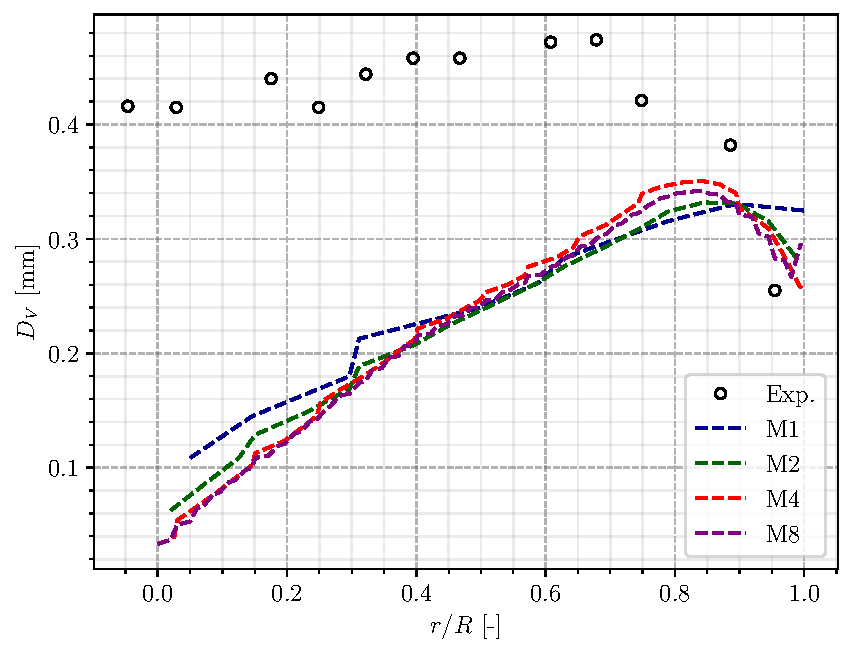
\includegraphics[width=0.5\linewidth]{img/DEBORA/cfd/30G2P26W16/30T66_dV_msh.pdf}
}
\\
\subfloat[Vapor velocity]{
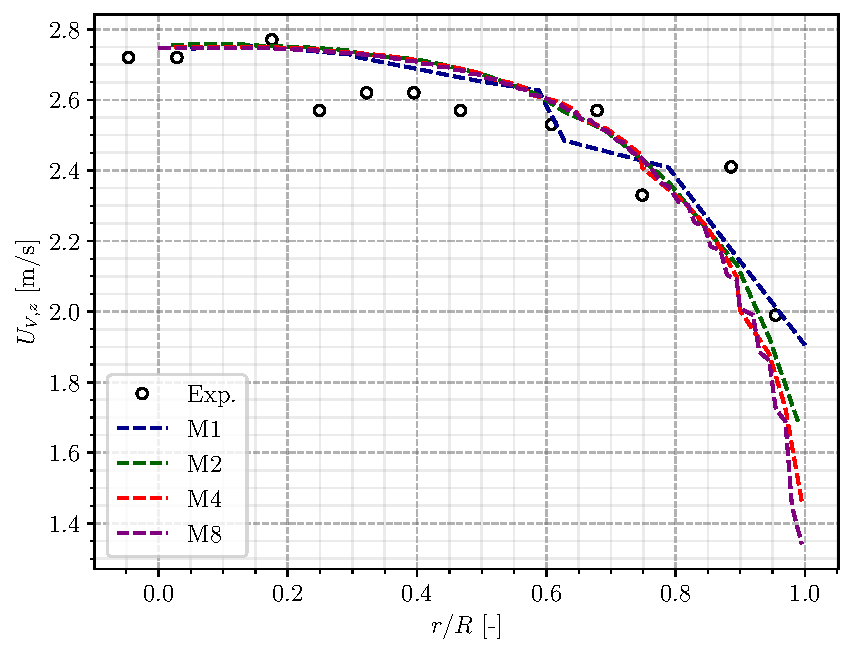
\includegraphics[width=0.5\linewidth]{img/DEBORA/cfd/30G2P26W16/30T66_Uvap_msh.pdf}
}
\subfloat[Liquid temperature]{
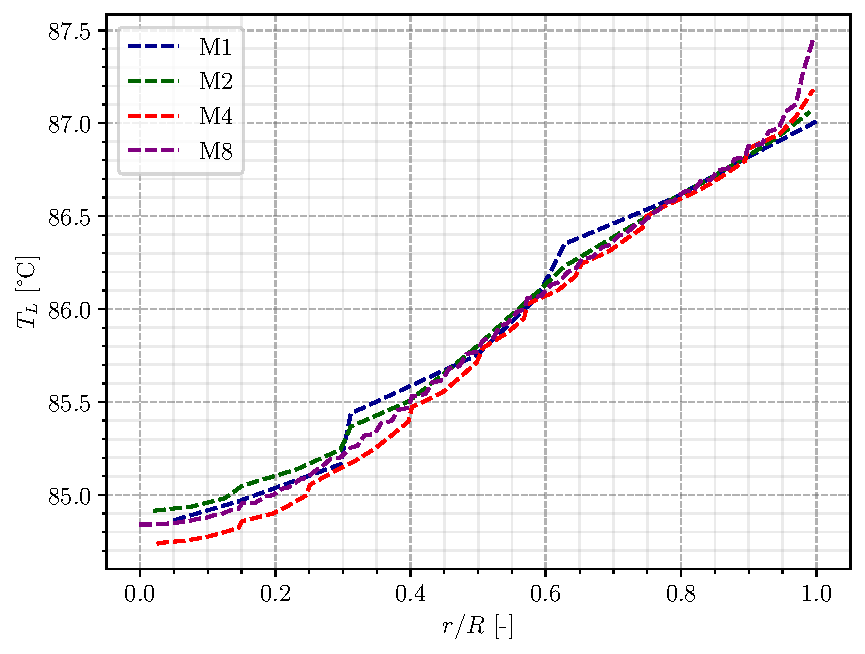
\includegraphics[width=0.5\linewidth]{img/DEBORA/cfd/30G2P26W16/30T66_TL_msh.pdf}
}
\caption{Mesh sensitivity study for 30G2P26Te66.6 case}
\label{fig:deb_cfd_msh_sensi}
\end{figure}


We see that the different meshes provide similar results for the void fraction, bubble diameter, vapor velocity and liquid temperature. This is particularly true for the M4 and M8 meshes, allowing to assume that an acceptable grid convergence is reached with the M4 mesh. \textbf{Therefore, further simulations will be conducted using the M4 mesh.}

\begin{remark*}
One of the most remarkable impact of the mesh concerns the liquid temperature in the wall-adjacent cell. As the mesh refines, the strong temperature gradient at the wall is logically better captured, inducing a net rise in the liquid temperature when $r/R \to 1$.
\end{remark*}



\section{C800 Cases Simulation : Thermal Measurements}

In this Section, we focus our attention on cases from the 8G2P26W16 series to assess liquid and wall temperature predictions. We sub-divide the case in three parts depending on the degree of subcooling at the outlet in order to cover both single-phase and fully boiling cases.



\subsection{High Subcooling Cases}

We start by simulating cases 8G2P26W16Te31.5 and Te44.9 which both have an outlet quality $x_{eq,out}<-0.25$, meaning that the fluid remains in its liquid phase along nearly the entire heating length. Results obtained for those cases are presented on Figure \ref{fig:deb_cfd_8T33_T44}.

\begin{figure}[!h]
\centering
\subfloat[Liquid temperature]{
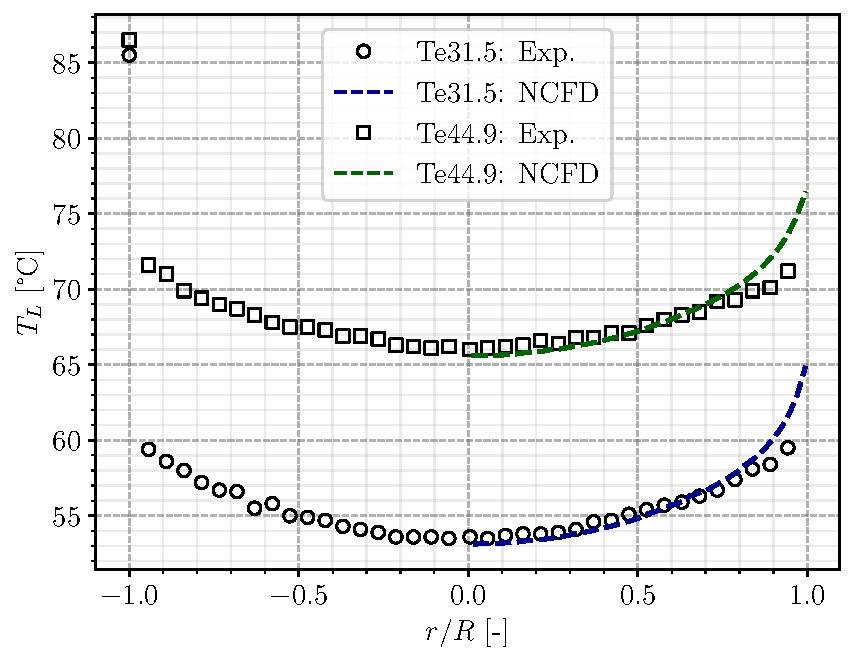
\includegraphics[width=0.4\linewidth]{img/DEBORA/cfd/8G2P26W16/8T31_T44_TL_ref.pdf}
\label{fig:8T31_T44_TL}
}
\subfloat[Wall temperature vs. axial position]{
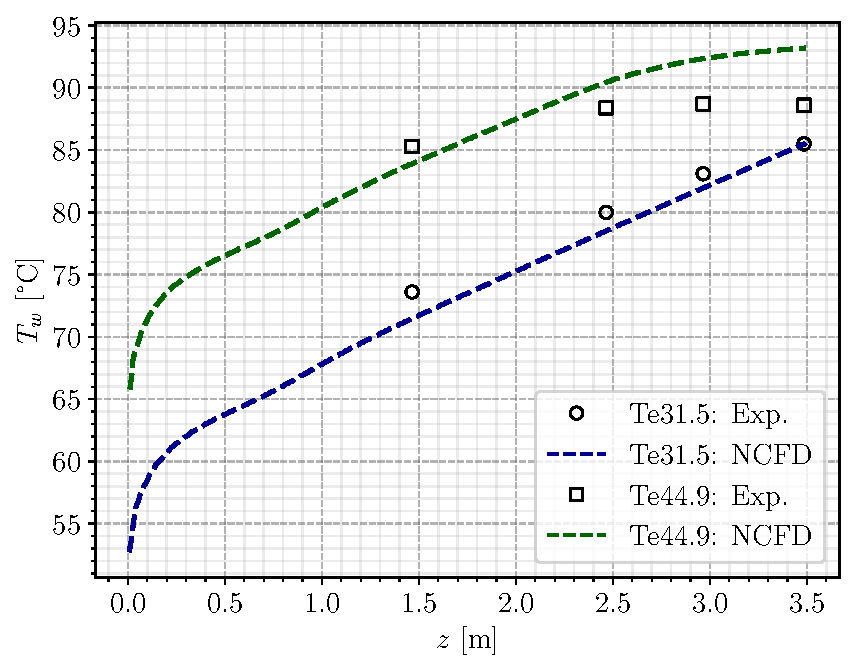
\includegraphics[width=0.4\linewidth]{img/DEBORA/cfd/8G2P26W16/8T31_T44_Tw_ref.pdf}
\label{fig:8T31_T44_Tw}
}
\\
\subfloat[Wall temperature vs. local quality]{
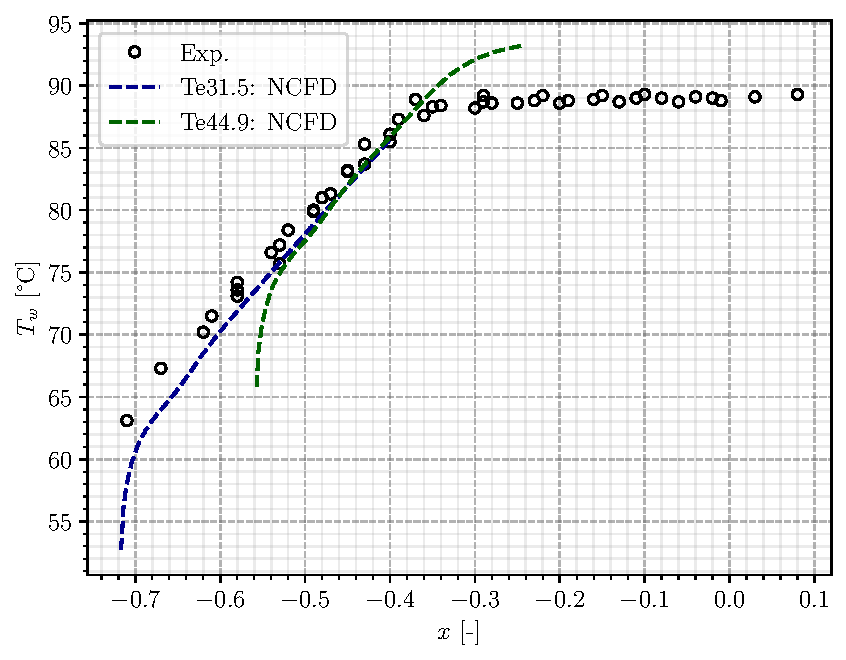
\includegraphics[width=0.4\linewidth]{img/DEBORA/cfd/8G2P26W16/8T31_T44_Tw_x_ref.pdf}
\label{fig:8T31_T44_Tw_x}
}
\caption{Simulation results for cases 8G2P26W16Te31. 5\& Te44.9}
\label{fig:deb_cfd_8T33_T44}
\end{figure}

\npar

The liquid temperature profiles are fairly reproduced with experimental the parabolic shape correctly captured along with quite precise prediction of the temperature values in the bulk (Figure \ref{fig:8T31_T44_TL}). Still, we note that an overestimation near the wall and a small underestimation (less than $1\degC$) when approaching the center of the pipe.

\npar

Wall temperature predictions in the single-phase region present a good agreement with the experimental measurements along the axial positions (Figure \ref{fig:8T31_T44_Tw}). This is further verified by transposition along the local quality $x_{eq}$ (Figure \ref{fig:8T31_T44_Tw_x}) gathering all the measurements from the 8G2P26W16 campaign, showing an average error of approximately $1 \degC$ up to $x_{eq} \approx -0.5$.

\npar

Those comparisons highlight the validation of the code for the single-phase flow part, implying that \textbf{the local liquid heat transfer coefficient (Eq. \ref{eq:ncfd_hfc}) is correctly computed along with a good heat transport along the radial direction}.


\subsection{Low Subcooling Cases}

Next cases to be simulated are 8G2P26W16Te55.7 and Te61.5. Their outlet quality is closer to saturation with $x_{eq,out} \geq -0.1$ and thus present a subcooled boiling region during a significant portion of the heating length. However, the bulk flow is expected to stay fully liquid in those conditions (Figure \ref{fig:G2P26W16_alpha}). The results are presented of Figure \ref{fig:deb_cfd_8T55_T61}.


\begin{figure}[!h]
\centering
\subfloat[Liquid temperature]{
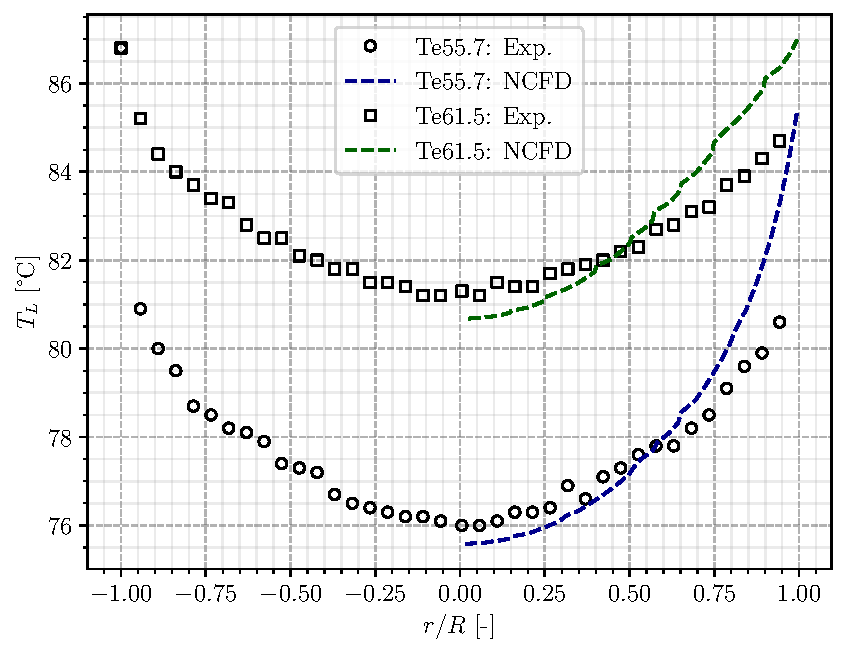
\includegraphics[width=0.4\linewidth]{img/DEBORA/cfd/8G2P26W16/8T55_T61_TL_ref.pdf}
\label{fig:8T55_T61_TL}
}
\subfloat[Wall temperature vs. axial position]{
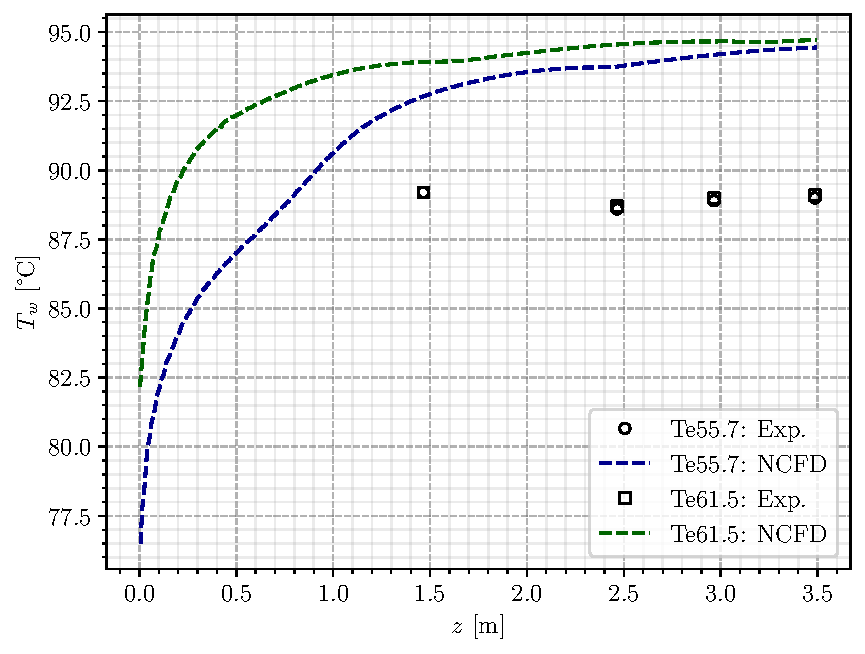
\includegraphics[width=0.4\linewidth]{img/DEBORA/cfd/8G2P26W16/8T55_T61_Tw_ref.pdf}
\label{fig:8T55_T61_Tw}
}
\\
\subfloat[Wall temperature vs. local quality]{
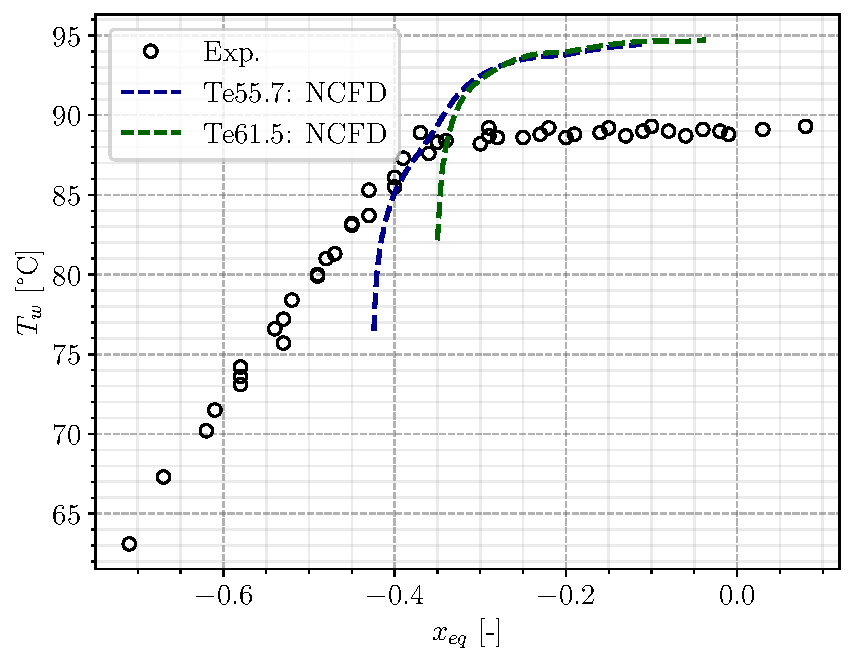
\includegraphics[width=0.4\linewidth]{img/DEBORA/cfd/8G2P26W16/8T55_T61_Tw_x_ref.pdf}
\label{fig:8T55_T61_Tw_x}
}
\caption{Simulation results for cases 8G2P26W16Te55.7 \& Te61.5}
\label{fig:deb_cfd_8T55_T61}
\end{figure}

\npar

Liquid temperature profiles (Figure \ref{fig:8T55_T61_TL}) are similar to those of the high subcooling cases (Figure \ref{fig:8T31_T44_TL}). The parabolic shape of the measurements is reasonably reproduced, with liquid temperature values close to the experiment. The same discrepancies are observed, namely a overestimation close to the wall and a small underestimation at the center (also lower than $1\degC$).

\npar

However, the wall temperature start to show significant discrepancies with the measurements (Figure \ref{fig:8T55_T61_Tw}). The deviation from the linear profile observed in the pure-single phase region towards a stabilization corresponding to the boiling regime fails to be reproduced (Figure \ref{fig:8T55_T61_Tw_x}). First, the temperature plateau appears to start later than the experiment (around $x_{eq}\approx -0.3$ for the simulations contrary to $x_{eq} \approx -0.4$ for the experiments) and further reaches a wall temperature up to $6 \degC$ above the measurements.

\npar
Albeit the liquid temperature seems correctly distributed along the radial direction in the subcooled boiling region (also meaning that any amount of vapor potentially produced at the wall is correctly re-condensed), the wall temperature behavior significantly deviates from the experiments both by missing the ONB and exhibiting a too large superheat in the boiling region. \textbf{This consequently casts interrogations towards the modeling of the wall temperature in the code, which is a result of the wall boiling model (Section \ref{sec:ncfd_HFP}).}



\subsection{Saturated Cases}

Finally, we focus on saturated cases 8G2P26W16Te66.6 and Te70.3, both having an outlet quality $x_{eq,out} > 0$. Under those operating conditions, uncondensed vapor is present in the bulk flow (Figure \ref{fig:G2P26W16_alpha}). Results of the simulation sfor those cases are presented on Figure \ref{fig:deb_cfd_8T66_T70}.



\begin{figure}[!h]
\centering
\subfloat[Liquid temperature]{
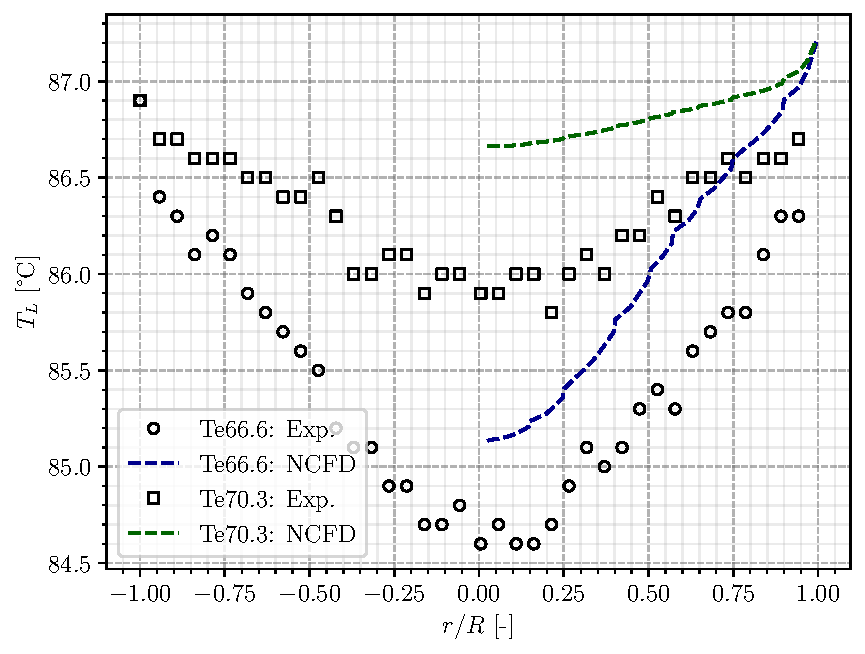
\includegraphics[width=0.4\linewidth]{img/DEBORA/cfd/8G2P26W16/8T66_T70_TL_ref.pdf}
\label{fig:8T66_T70_TL}
}
\subfloat[Wall temperature vs. axial position]{
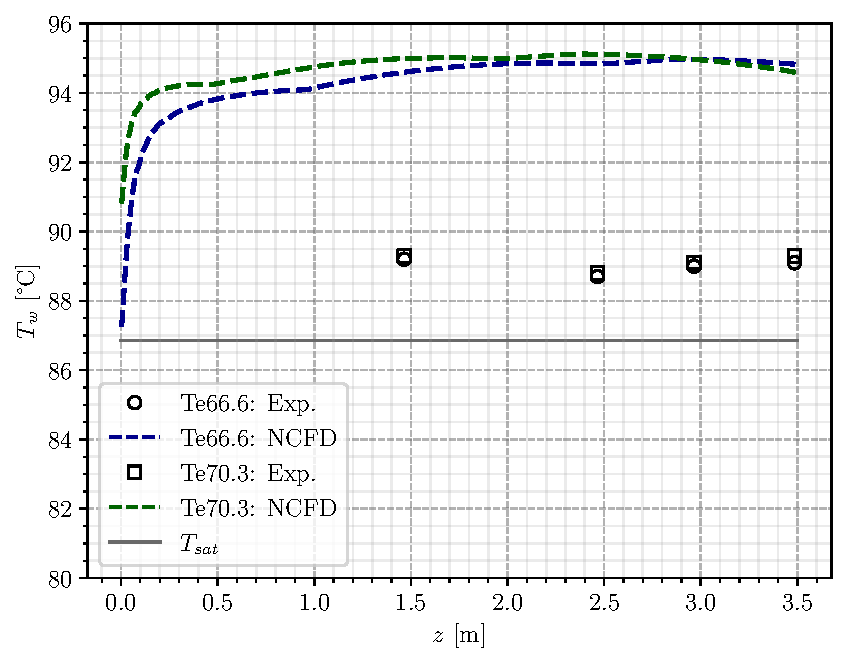
\includegraphics[width=0.4\linewidth]{img/DEBORA/cfd/8G2P26W16/8T66_T70_Tw_ref.pdf}
\label{fig:8T66_T70_Tw}
}
\\
\subfloat[Wall temperature vs. local quality]{
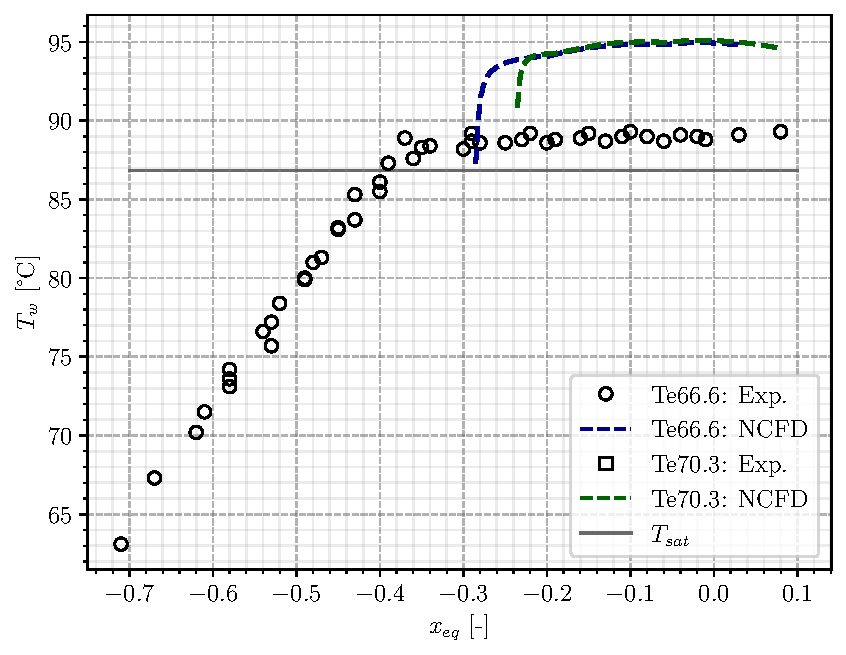
\includegraphics[width=0.4\linewidth]{img/DEBORA/cfd/8G2P26W16/8T66_T70_Tw_x_ref.pdf}
\label{fig:8T66_T70_Tw_x}
}
\caption{Simulation results for cases 8G2P26W16Te66.6 \& Te70.3}
\label{fig:deb_cfd_8T66_T70}
\end{figure}


Contrary to previous observations in subcooled cases, the liquid temperature profiles (Figure \ref{fig:8T66_T70_TL}) are are overestimated over the whole radial section for both cases. The shape exhibited are however similar to the experiments, with a flattening of the liquid temperature for the Te70.3 case.

\npar

In those conditions, boiling starts immediately at the beginning of the heated length. Therefore, wall temperature is expected to rapidly stabilize to the boiling temperature, which is actually what happens in the simulations (Figure \ref{fig:8T66_T70_Tw})). As previously noted for the low subcooling cases, the wall temperature during boiling is overestimated by approximately $6\degC$. 

\npar

Those saturated cases are confirming that \textbf{the boiling model fails to predict the wall temperature}. Moreover, the small yet observed 


\clearpage









In this work, we present the simulations of the following cases:
\begin{itemize}
\item C8G2P26W16Te44.9 and C8G2P26W16Te49.6 (single-phase flow)
\item C8G2P26W16Te66.6 and C8G2P26W16Te70.3 (two-phase flow)
\item C30G2P26W16Te66.6 and C30G2P26W16Te70.6 (two-phase flow)
\end{itemize}

The pressure of $26~\text{bar}$ is chosen to match the pressure of the mixing vanes cases (DEBORA-Promoteur, Section \ref{sec:deb_prom}). Mesh sensitivity is performed over two meshes: a large mesh (M1) with $460~356\text{ cells }=338\text{ radial } \times 1362 \text{ axial cells}$ and a fine mesh (M2) with $3~157~952\text{ cells }=1568\text{ radial } \times 2014 \text{ axial cells}$.

On Figure \ref{fig:th_1phi_res}, we present the results regarding liquid temperature at the outlet and wall temperature. The liquid temperature profile seems to be correctly reproduced by the simulations, though we see a slight overestimation close to the wall. Looking closer at boiling cases shows a difference of $\approx 0.5\degree$ C, which is close to the uncertainty of the measurements \cite{garnier_local_2001}. Concerning the wall temperature, it appears that it is underestimated before the \textbf{Onset of Nucleate Boiling} (ONB) ($T_{w}<T_{sat}$) and overestimated after the ONB ($\approx +5\degree$C). Post-ONB wall temperature is characterized by a stabilization of its value above the saturation temperature (here $T_{w,ONB}-T_{sat}\approx 2\degree\text{C}$).

%
\begin{figure}[h!]
\centering
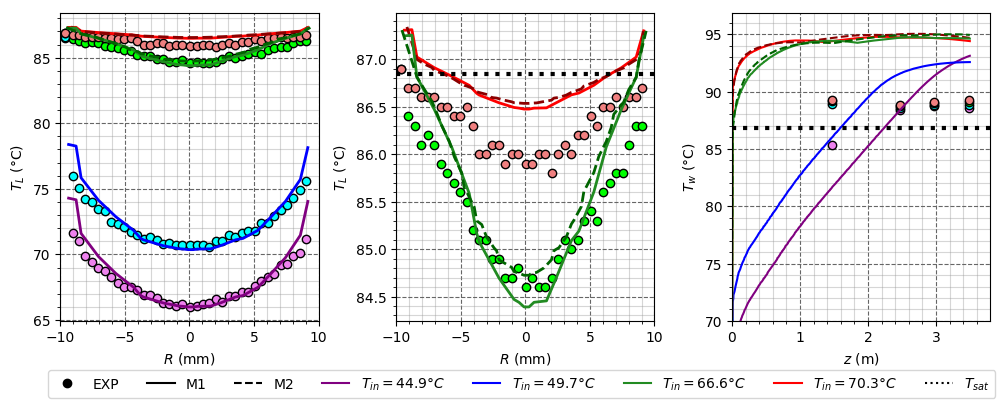
\includegraphics[scale=0.60]{img/DEBORA/c8.png}
\caption{NCFD (lines) vs. Exp. (circles) - $T_{L}$ and $T_{w}$ - Cases C8G2P26W16Te44.9, Te49.6, Te66.6 and Te70.3 - Simulations using two meshes M1 (coarse) and M2 (fine).}
\label{fig:th_1phi_res}
\end{figure}
%

%%
%\begin{figure}[!htb]
%\vspace{16pt}
%\begin{spacing}{1.0}
%\centering
%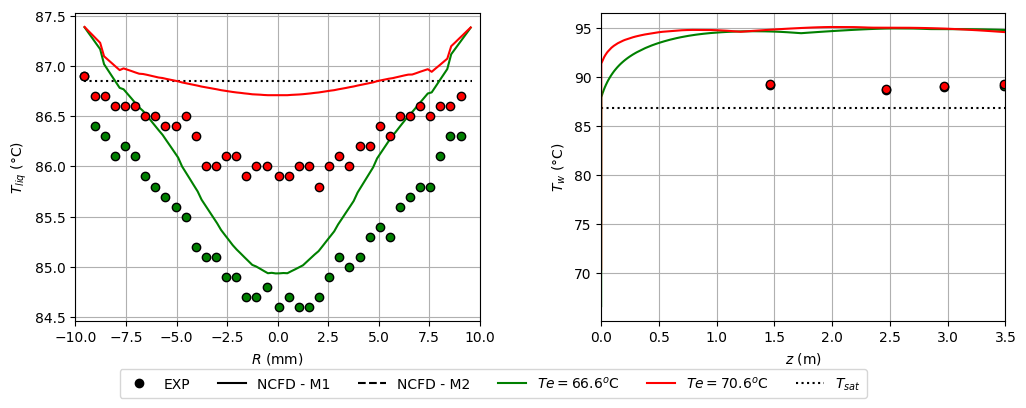
\includegraphics[scale=0.60]{img/DEBORA/thermal_diph.png}
%\caption{NEPTUNE\_CFD simulations results vs. experimental measurements - $T_{L}$ and $T_{w}$ - Cases C8G2P26W16Te66.6 and C8G2P26W16Te70.3}
%\label{fig:th_diph_res}
%\end{spacing}
%\vspace{16pt}
%\end{figure}
%%



%
\begin{figure}[h!]
\centering
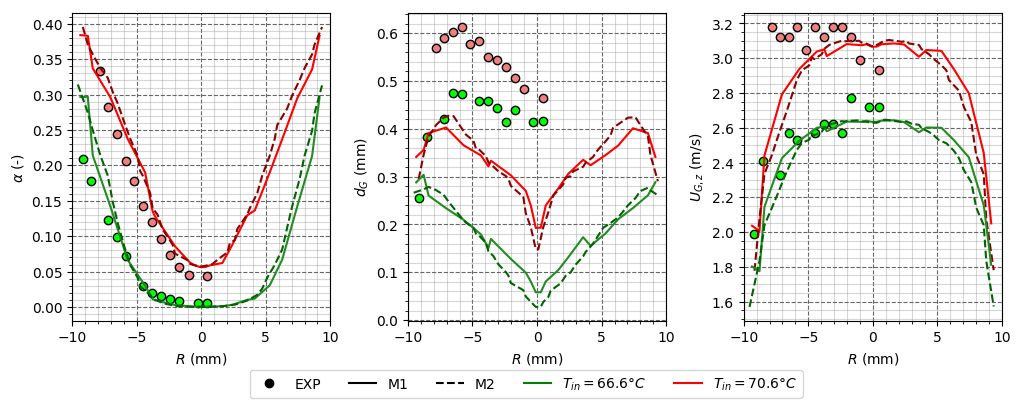
\includegraphics[scale=0.60]{img/DEBORA/c30.png}
\caption{NCFD (lines) vs. Exp. (circles) - $\alpha$, $d_{G}$ and $U_{G,z}$ - Cases C30G2P26W16Te66.6 and Te70.6 - Simulations using two meshes M1 (coarse) and M2 (fine).}
\label{fig:topology_res}
\end{figure}
%

On Figure \ref{fig:topology_res}, we compare the results of the simulations to the experiments regarding void fraction, bubble Sauter diameter and axial gas velocity. Void fraction profiles are quite correctly reproduced, though we observe a $10\%$ higher peak at the wall for $T_{in}=66.6\degree$C. The order of magnitude of bubble diameter is correct ($\sim 0.1\text{mm}$) and NEPTUNE\_CFD manages to detect coalescence (increase of bubble diameter when leaving the wall) and bulk condensation (decrease of bubble diameter when reaching the core of the flow), which is in qualitative agreement with the experiments. Quantitatively speaking, bubble diameter is globally underestimated. Finally, gas velocity profile is reasonably reproduced for $T_{in}=66.6\degree$C, but not for $T_{in}=70.6\degree$C. The latter experimental profile is flatter, which could be explained by a change of flow regime since uncondensed vapor is detected in the bulk.  

Finally, the simulations reasonably agree with the experiments. The strongest discrepancies being mostly the wall temperature and bubble diameter. Potential ways of improving those results are investigated in next sub-section.

\subsection{Investigating the nucleation site density modeling $N_{sit}$}

In NEPTUNE\_CFD, wall temperature is computed through the Heat Flux Partitioning model, which role is to find the appropriate $T_{w}$ which balances Equation $\ref{eq:HFP}$. However, some laws used to express parameters such as $N_{sit}$, $f$, or $d_{d}$ are quite old and simple. For instance, the {Lemmert} \& {Chawla}\cite{lemmert_influence_1977} expression of $N_{sit}$ only depends on the wall superheat (Sub-section \ref{subsec:HFP}).%, meaning that it can not reproduce potential influence of the pressure on the nucleation site density.

A comparison of the {Lemmert} \& {Chawla} law\cite{lemmert_influence_1977} with  the {Hibiki} \& {Ishii}\cite{hibiki_active_2003} law for $N_{sit}$ against 4 data sets from the literature is presentend on Figure \ref{fig:nsit}. The {Hibiki} \& {Ishii} correlation depends simultaneously on wall superheat, pressure and contact angle.  Experimental measurements of {Borishanskii} \etal\cite{borishanskii_heat_1969}, {Richenderfer} \etal\cite{richenderfer_investigation_2018}, {Kossolapov} \etal\cite{kossolapov_experimental_2021} and {Zhou} \etal\cite{zhou_experimental_2020-1} are used to assess the two nucleation site density correlations.
%
\begin{figure}[h!]
\centering
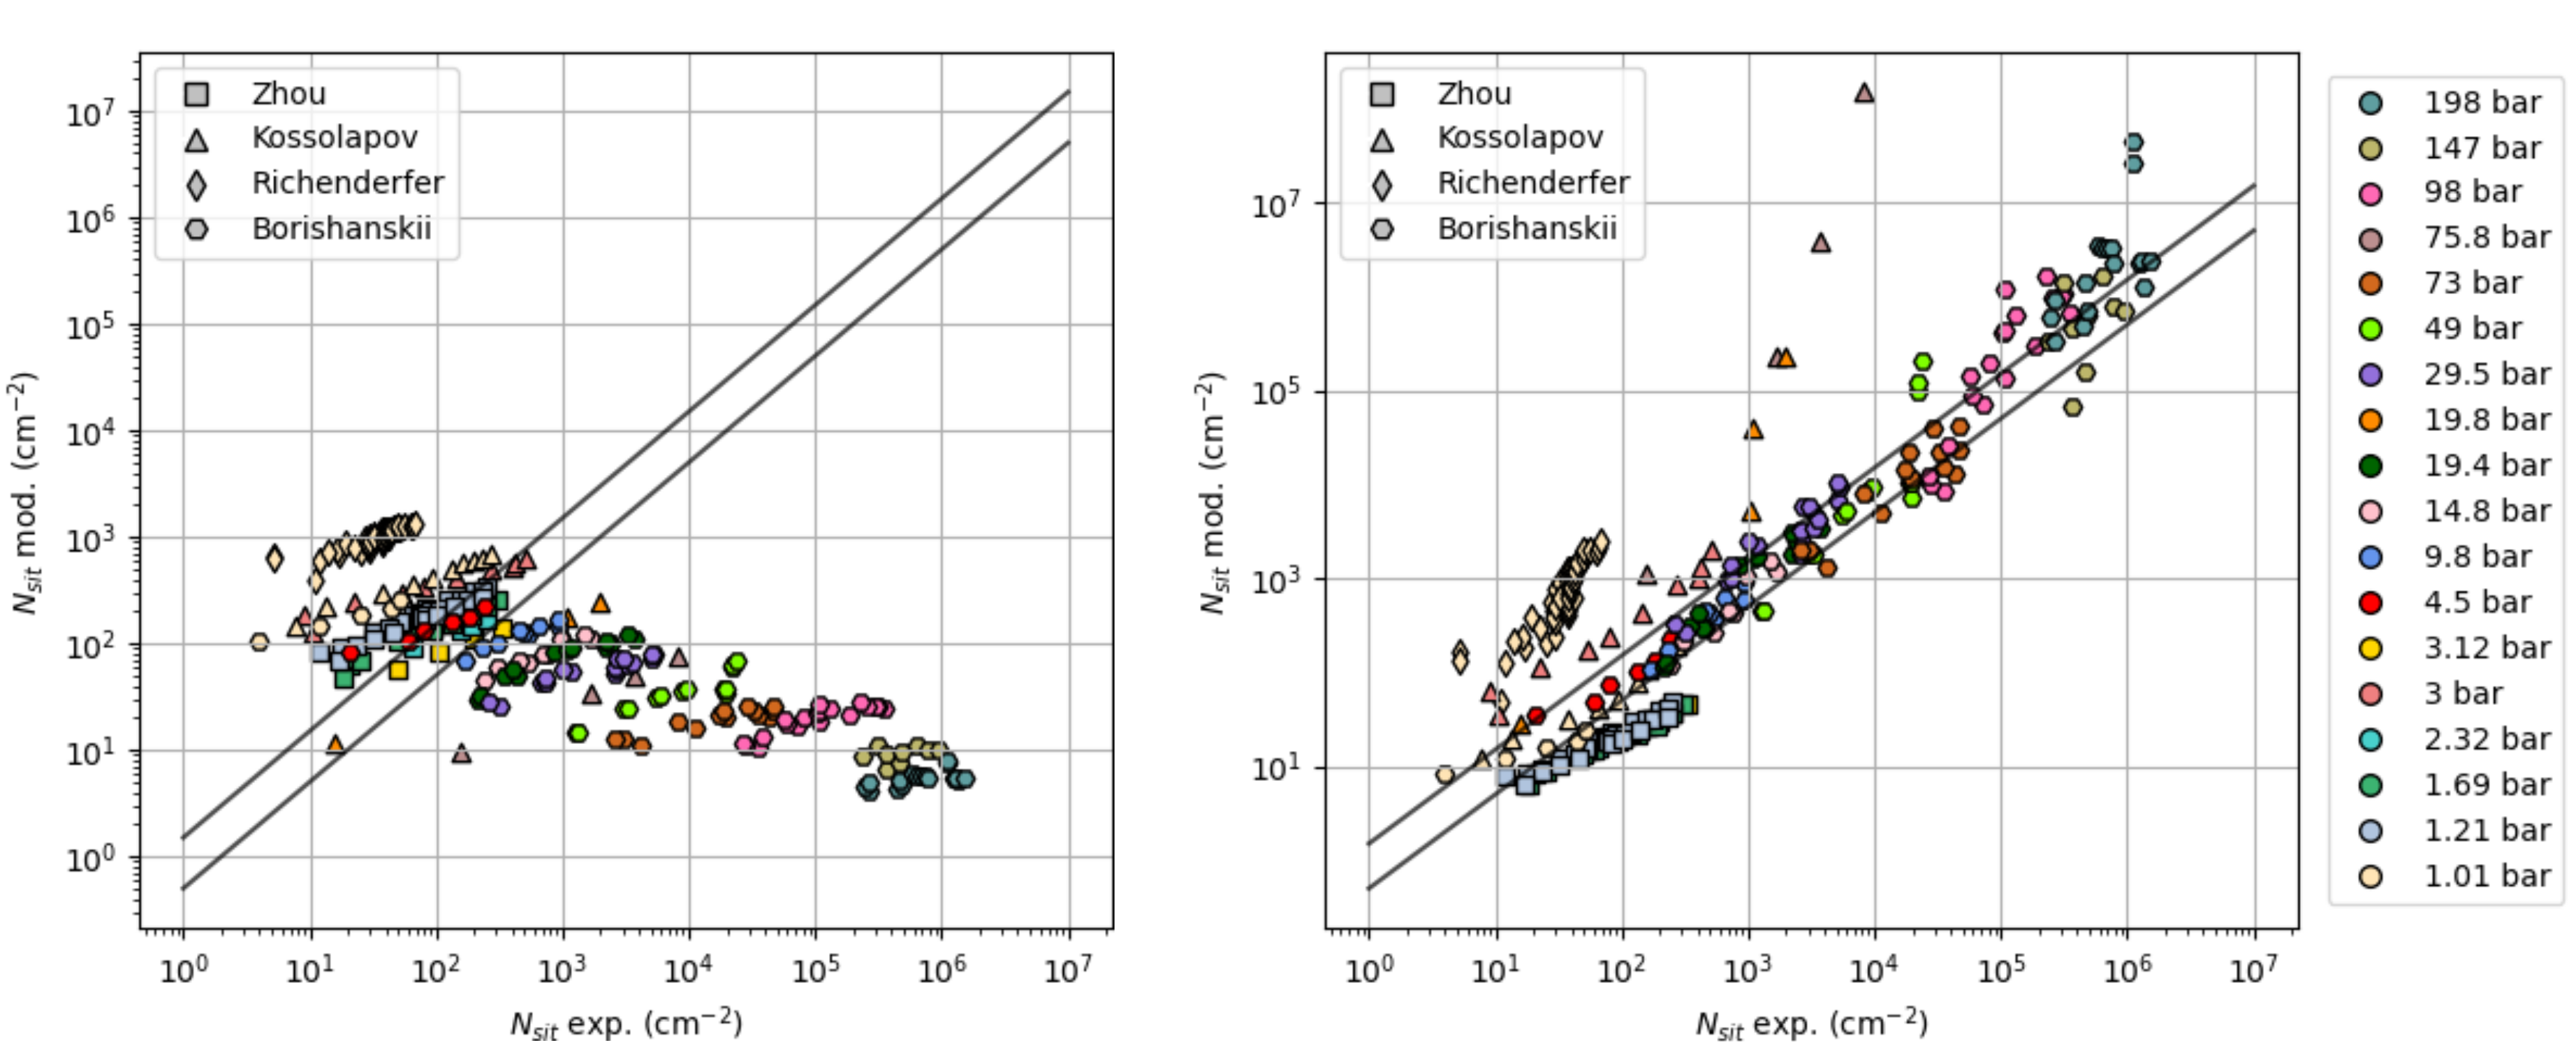
\includegraphics[scale=0.45]{img/DEBORA/nsit.png}
\caption{$N_{sit}$ correlations of {Lemmert} \& {Chawla} (left) and {Hibiki} \& {Ishii} (right) vs. exp. data from literature. Operation pressures are displayed. $\pm 50\%$ error bars are drawn in black.}
\label{fig:nsit}
\end{figure}
%

Figure \ref{fig:nsit} clearly shows that the {Lemmert} \& {Chawla} law lack of pressure dependence fails to reproduce high pressure measurements contrary to the {Hibiki} \& {Ishii} one. Even though {Hibiki} \& {Ishii} correlation shows significant discrepancies with measurements of {Kossolapov} \etal and {Richenderfer} \etal, its prediction capability is greater in average than {Lemmert} \& {Chawla} correlation.

%
\begin{figure}[h!]
\centering
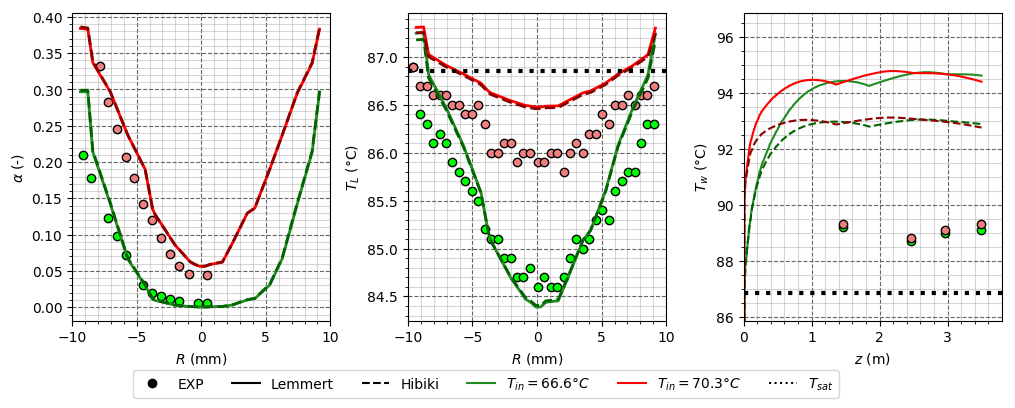
\includegraphics[scale=0.60]{img/DEBORA/plot_HI.png}
\caption{NCFD results for $\alpha$, $T_{L}$ and $T_{w}$ using {Lemmert} \& {Chawla} and {Hibiki} \& {Ishii} correlation. Cases 8G2P26W23Te66.6 and Te70.3, 30G2P26W23Te66.6 and 70.6.}
\label{fig:NCFD_nsit}
\end{figure}
%
To assess the influence of nucleation site density law on NEPTUNE\_CFD computations, we compare results obtained with both correlations on Figure \ref{fig:NCFD_nsit}, which shows a remarkable impact of the modification of $N_{sit}$ correlation. Using {Hibiki} \& {Ishii} correlation reduces the error on $T_{w}$ by approximately $2\degree\text{C}$ while $\alpha$ and $T_{L}$ remain unchanged. This implies that the same heat flux partitioning is found with the two models, but that the pressure dependence of {Hibiki} \& {Ishii} law helped to balance Equation \ref{eq:HFP} using a lower $T_{w}$, thus closer to experimental measurements.

Such a result indicates that the HFP model could be improved through a systematic analysis of each parameter's impact and modeling (bubble departure diameter, detachment frequency, etc.). Assembling a more recent and consistent model could provide better results regarding wall temperature prediction. Models such as the one developed by {Kommajosyula}\cite{kommajosyula_development_2020} could be interesting to apply for high-pressure flows.


Now that simple tube boiling flow has been assessed through the presented results, next section will focus on the simulation of boiling flow in a tube equipped with a mixing device.% using DEBORA-Promoteur experimental results.